\problemname{Tivoli}

Lisa er kommet til Tivoli og har bestemt sig for at prøve $N$ forlystelser en gang hver.
Hver forlystelse er anlagt to gange, og de to anlæg er lige gode; totalt findes der altså $2N$ anlæg.
Givet positionerne for samtlige anlæg hjælp Lisa med at planlægge, hvilke $N$ anlæg hun skal vælge og i hvilken rækkefølge for at minimere den strækning, hun skal gå for at besøge alle $N$ forlystelser.

Desuden begynder og slutter hun ved indgangen. Indgangen er i origo, $(0,0)$.

\begin{figure}[h]
    \centering
    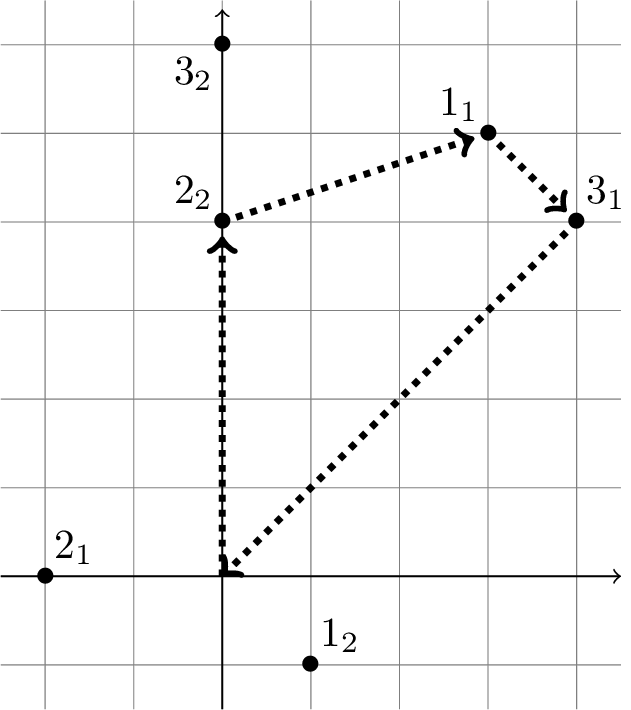
\includegraphics[width=0.2\textwidth]{tivoli}
    \caption{En illustration av det första exempelfallet och en optimala lösningen.}
\end{figure}

\section*{Indlæsning}
Første linje består af heltallet $N$, som angiver antallet af forlystelser, som Lisa vil besøge ($1 \le N \le 15$).
Derefter følger $N$ linjer, hvoraf første linje beskriver forlystelse  nummer~$1$, anden linje beskriver forlystelse nummer $2$, osv.
Hver linje indeholder fire heltal: $x$- og $y$-koordinaterne for denne forlystelses første anlæg efterfulgt af $x$- og $y$-koordinaterne for denne forlystelseforlystelses anlæg.
Koordinaternes absolutværdi er mindre end en million.

Intet anlæg er på samme plads som noget andet.
Intet anlæg er i origo.

\section*{Udskrift}
Udskriftens første linje skal bestå af et decimaltal skrevet med decimalpunktum: hvor langt Lisa skal gå. 
Derefter skal der komme $N$ linjer med to heltal på hver, forlystelsesnummeret (mellem $1$ og $N$) og anlægsnummeret ($1$ eller $2$).

Den første af de $N$ linjer fortæller altså, hvilket anlæg hun skal besøge først, og den sidste linje fortæller, hvilket anlæg hun skal besøge sidst.
Hvis der findes flere veje med lige kort strækning (fx ved at følge en løsning baglæns), kan du vælge hvilken som helst af dem.
Læg mærke til at det først udskrevne decimaltal skal tage hensyn til, at Lisa skal begynde og slutte ved indgangen.

Den relative eller absolutte fejl skal være mindre end $10^{-5}$.

\section*{Pointgivning}
Din løsning bliver kørt på seks grupper af test. For at få point for en gruppe, skal du klare alle test i gruppen.

\noindent
\begin{tabular}{| l | l | p{12cm} |}
  \hline
  Gruppe & Point & Begrænsninger \\ \hline
  $1$    & $20$        & $N \le 1$ \\ \hline 
  $2$    & $40$        & $N \le 5$ \\ \hline
  $3$    & $40$        & Ingen yderligere begrænsninger. \\ \hline 
\end{tabular}
